\chapter{Proposed Approach}
\begin{itemize}
\item describe everything you yourself did (as opposed to the fundamentals chapter, which explains what you built on)
\item start with a theoretical approach
\item describe the developed system/algorithm/method from a high-level point of view
\item go ahead in presenting your developments in more detail
\item recommended length: approximately one third of the thesis.
\end{itemize}

Starting from the ESP-Now protocol, different approaches can be chosen to route the control signals to the fixtures. 
In the following I will present different approaches, which are also investigated experimentally.

\section{Design}
\label{sec:design}
\begin{itemize}
	\item Specification of the protocols
	\item analytic results (simulierte Ergebnisse)
	\item Ad-Hoc complexity of topology is not a problem, because of its simple star structure.
\end{itemize}

In this chapter there are different approaches presented and discussed.
There are several specifications to go through and some details of the implementation.

\subsection{Slim Unicast}
\begin{itemize}
\item topology
\item Network stack
\item re transmissions
\item reliability
\item tolja calculation sheet for 802.11
\item wireshark measurements
\end{itemize}

Art-Net \cref{sec:artnet} makes use of the \ac{IP} and the \ac{UDP} for routing and controlling the transmissions.
The most similar approach using ESP-Now insted of Art-Net is cutting the Layer above the Data Link Layer.
It is more like a direct transmission between sender and fixture, saving some overhead.
In the Application layer is the Art-Net replaced with the Slim-Unicast, controlling the order and timing of the repetitions.
\todo{ist Slim-Unicast auf sender-seite nicht anders zu behandeln als auf empfängerseite?}

\begin{table}[h]
	\centering
	% \label{tab:layer_overview}
	\begin{tabular} { ccc }
		\begin{tabular}{ |c| } 
			\hline
			Art-Net\\
			\hline
			UDP\\
			\hline
			IP\\
			\hline
			802.11 DL/Unicast\\
			\hline
			802.11b/g/n PHY\\ 
			\hline
		\end{tabular}
		\begin{tabular}{ |c| } 
			\hline
			Slim-Unicast\\
			\\
			\\
			\hline
			802.11 DL/Unicast\\
			\hline
			802.11b/g/n PHY\\ 
			\hline
		\end{tabular}
		\begin{tabular}{ |c| } 
			\hline
			Slim-Broadcast\\
			\\
			\\
			\hline
			802.11 DL/Broadcast\\
			\hline
			802.11b/g/n PHY\\ 
			\hline
		\end{tabular}
	\end{tabular}
	\caption{OSI Layer of Slim Unicast and Broadcast}
	\label{tab:Layer}
\end{table}
\TODO{Fehlt hier nicht ESP-Now?}

An intuitive way is to send the most recent signal to all fixtures via Round Robin.
The sender node selects a fixture after each other and transmits all the needed channel to it.
\TODO{Discuss the inimportance of order of round robin in unicast}
\TODO{calculation of the estimated transmission time of unicasts}
One benefit of the unicast is the support of acknoledgements. So the reliability should be very good. 
Unfortunately the ESP-Now protocol does not allow to control the number of retransmissions before the packet is discarded.
Synchronisation of all devices is also expensive, because every fixture has to wait after the successfull receiving of his packet until the last fixture received his packet too.
This is further discussed in \cref{sub:DelayedRepetition}.
\TODO{move to buffering delay??}

\begin{align*} \label{eq:transmission_unicast}
	t_{bestcase}  &= N \cdot (t_{transmission} + 8 \cdot t_{ack}) \\
	t_{worstcase} &= N \cdot (t_{transmission} + 1 \cdot t_{ack})
\end{align*} 

The idea of the unicast is, that a transmission to each device is very fast, because the transmitted payload is very small (1-25 Byte).
However, since we are sending many small packets, it can be assumed that we will be sending a lot of overhead.
So we playing off reliability against transmission speed.
\todo{Man kann transmissions skippen, wenn eine fixture keine veränderten daten erhält}

\todo{reference to unicast topolgy in fundamentals}

\subsection{Slim Broadcast}
\begin{itemize}
	\item topology
	\item efficiency
	\item for how many nodes it does make theoretical a difference
\end{itemize}

The ESP-Now protocol supports both unicast and broadcast.
Instead of transmitting every unicast after each other, we transmit a broadcast with the payload of all channels at the same time to all fixtures.
If we need more than 250 channel we have to send to broadcasts to transmit all information to all fixtures.
To achieve this we need to tell each fixture in advance his channel.
A fixture with a channel above 250 needs to modulo to get the broadcast ID.

\TODO{Notwendig?}
\begin{align*}
	315 \mod 250 &= 1 \\
	315 / 250 &= 65
\end{align*}

Insead of transmitting to several fixtures after each other we just transmitt to all fixtures at the same time.
This solves the problem of synchronization for less than 250 channel.
For more than 250 each fixture has to wait until the last broadcast is arrived, 
even if he must be discarded because the required channel has already been arrived in a previous broadcast.
Through less overhead there is an estimated difference when a specific amount of fixtures is reached.
\TODO{Grafik die zeigt, wie der Broadcast besser performt, sobald eine bestimmte zahl fixtures erreicht ist}

\begin{figure}
	\centering
	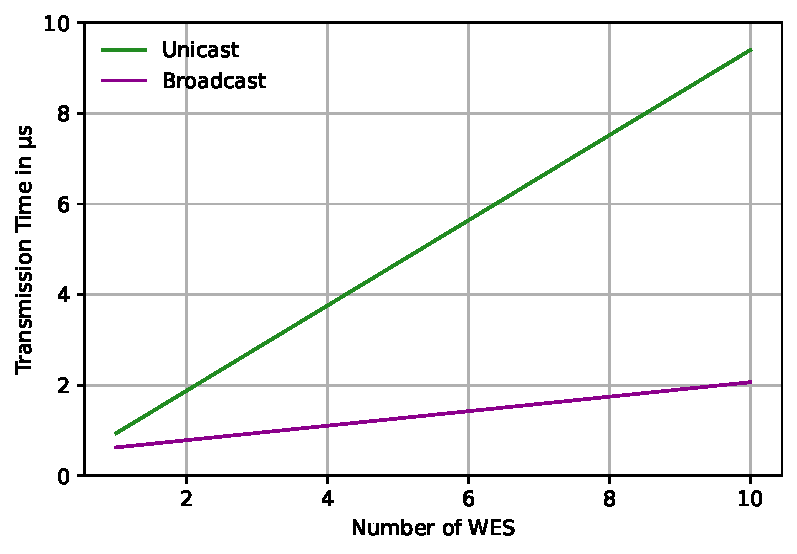
\includegraphics[scale=0.7]{/home/walther/Documents/bachelor/Plot2/Graphs/bc_uc_transmissiontime_analytic.pdf}
	\caption{Transmission Time of Unicast vs Broadcast}
	\label{fig:bc_uc_transmissiontime_analytic}
\end{figure}

\begin{figure}
	\centering
	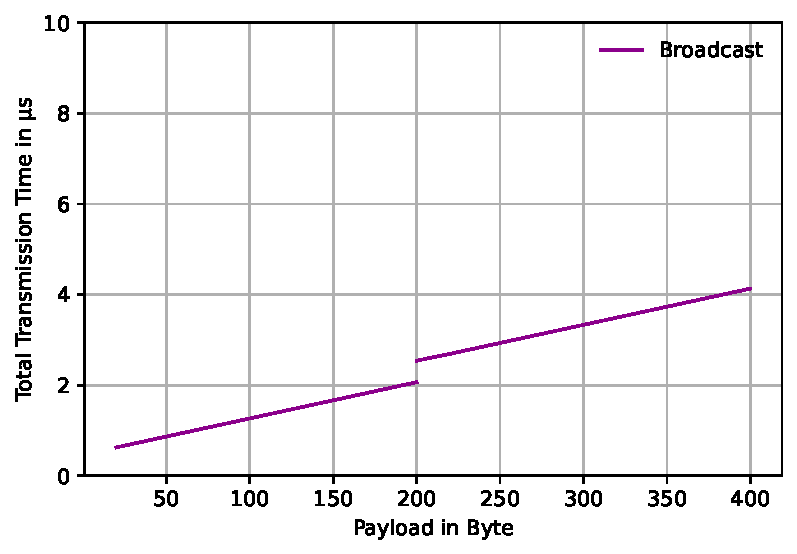
\includegraphics[scale=0.7]{/home/walther/Documents/bachelor/Plot2/Graphs/bc_analytic.pdf}
	\caption{Transmission Time of Unicast vs Broadcast Analytis}
	\label{fig:bc_analytic}
\end{figure}

\subsection{Rapid Repetition}
\begin{itemize}
\item simple
\item redundant
\item fast
\item cite paper from tolja
\item explain why its only relevant for BC?
\end{itemize}

The ESP-Now broadcast does not support acknoledgements.
So we can't retransmit a packet to the fixture, which is not arrived successfully.
In case of broadcast we had to transmit the hole broadcast or an unicast to each fixture wich does not send back the acknoledgement.\\

Since this is very cumbersome to implement, it is a good approach to simply repeat each broadcast. 
\TODO{Cite paper A First Implementation and Evaluation of the IEEE 802.11aa Group Addressed Transmission Service}
This is called rapid repetition. \TODO{Is Rapid Repetition a appropriate name? Unsosliced Repetition is better siehe Paper?}
The idea is, that we can push the reliability wich each redundant retransmission.

The estimated reliability of a fixture with average success ratio (SR) of 83\% without Repetition has to be 83\%.
If we increase the number of Rapid Repetitions (RR) we can roughly estimate:
\begin{align}
	% ER &= 1-SR &\text{Errorrate}\\
	SR_{RR}(RR) &= 1-(1-SR)^{RR+1} 
\end{align}
\todo{RR von 0 beginnen}
\TODO{grafische Darstellung RR=[0,1,2,3,4], für einen guten und einen schlechten Knoten 83\% und 95\%}

\begin{figure}
	\centering
	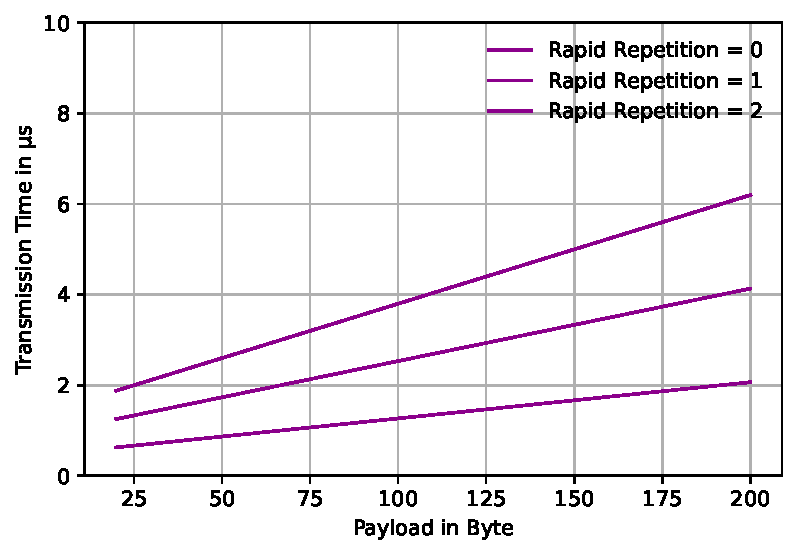
\includegraphics[scale=0.7]{/home/walther/Documents/bachelor/Plot2/Graphs/rr_transmission_time.pdf}
	\caption{Transmission Time with with different \ac{RR}s}
	\label{fig:bc_analytic}
\end{figure}

We have to figure out how many repetitions we should transmit in order to find the best balance between reliability and latency/update ratio.
This hardly correlates with the overall success ratio in the (test-)setup. \TODO{(test-)setup: kann man das so schrieben?}

\subsection{Delayed Repetition}
\label{sub:DelayedRepetition}
\begin{itemize}
\item when to perform repetition
\item buffering delay
\item explain why its only relevant for BC?
\end{itemize}

To push the idea of rapid repetion even further, we should take a look to temporarily occuring disturbances.
\TODO{Figure of bad channel time}

\section{Implementation}
\begin{itemize}
\item ESP programming
\item code examples
\item python script
\end{itemize}

\todo{for later use: ESP-NOW User Guide, V1, source: \url{https://www.espressif.com/en/support/documents/}}

\subsection{ESP Programming}
\begin{itemize}
\item broadcast unicast
\item IDF/Arduino
\item IDE \& ESP hardware flashing
\item setup devices
\end{itemize}
Unfortunally in the documentation of the ESP-protocol is written, that broadcast is not supported 
% \TODO{link, https:\/\/www.espressif.com\/sites\/default\/files\/documentation\/esp-now_user_guide_en.pdf, 2016}
but actually it is. Insted of adding the \ac{MAC} Address of a fixture, we can use 
\todo{has this a proper name, like broadcast address?} ff:ff:ff:ff:ff:ff 
to add a peer with the broadcast \ac{MAC}.

\label{lst:shorttable}
\begin{lstlisting}
void addFixtureToPeerList(const uint8_t *mac_addr) 
{
	if (esp_now_is_peer_exist(mac_addr)) return;

	peer_info.channel = 1;               // 1-14
	peer_info.ifidx   = ESP_IF_WIFI_STA; // Station mode
	peer_info.encrypt = false;         	 // not needed
	memcpy(peer_info.peer_addr, mac_addr, 6);

	esp_err_t status = esp_now_add_fixture(&peer_info);
	if (ESP_OK != status) 
	{
		Serial.println("[ERROR] Could not add fixture");
	}
	else 
	{
		Serial.println("[OK] fixture added");
	}
}
\end{lstlisting}
% \lstinputlisting[caption=Scheduler, style=customc]{hello.c}

\TODO{fix colorscheme omf code examples}

\subsection{Collecting measurment results}
\begin{itemize}
\item Collecting values
\item state machine
\item python script
\item saving values
\item digital encoding e.g.: 777477472717
\end{itemize}

\begin{figure}
	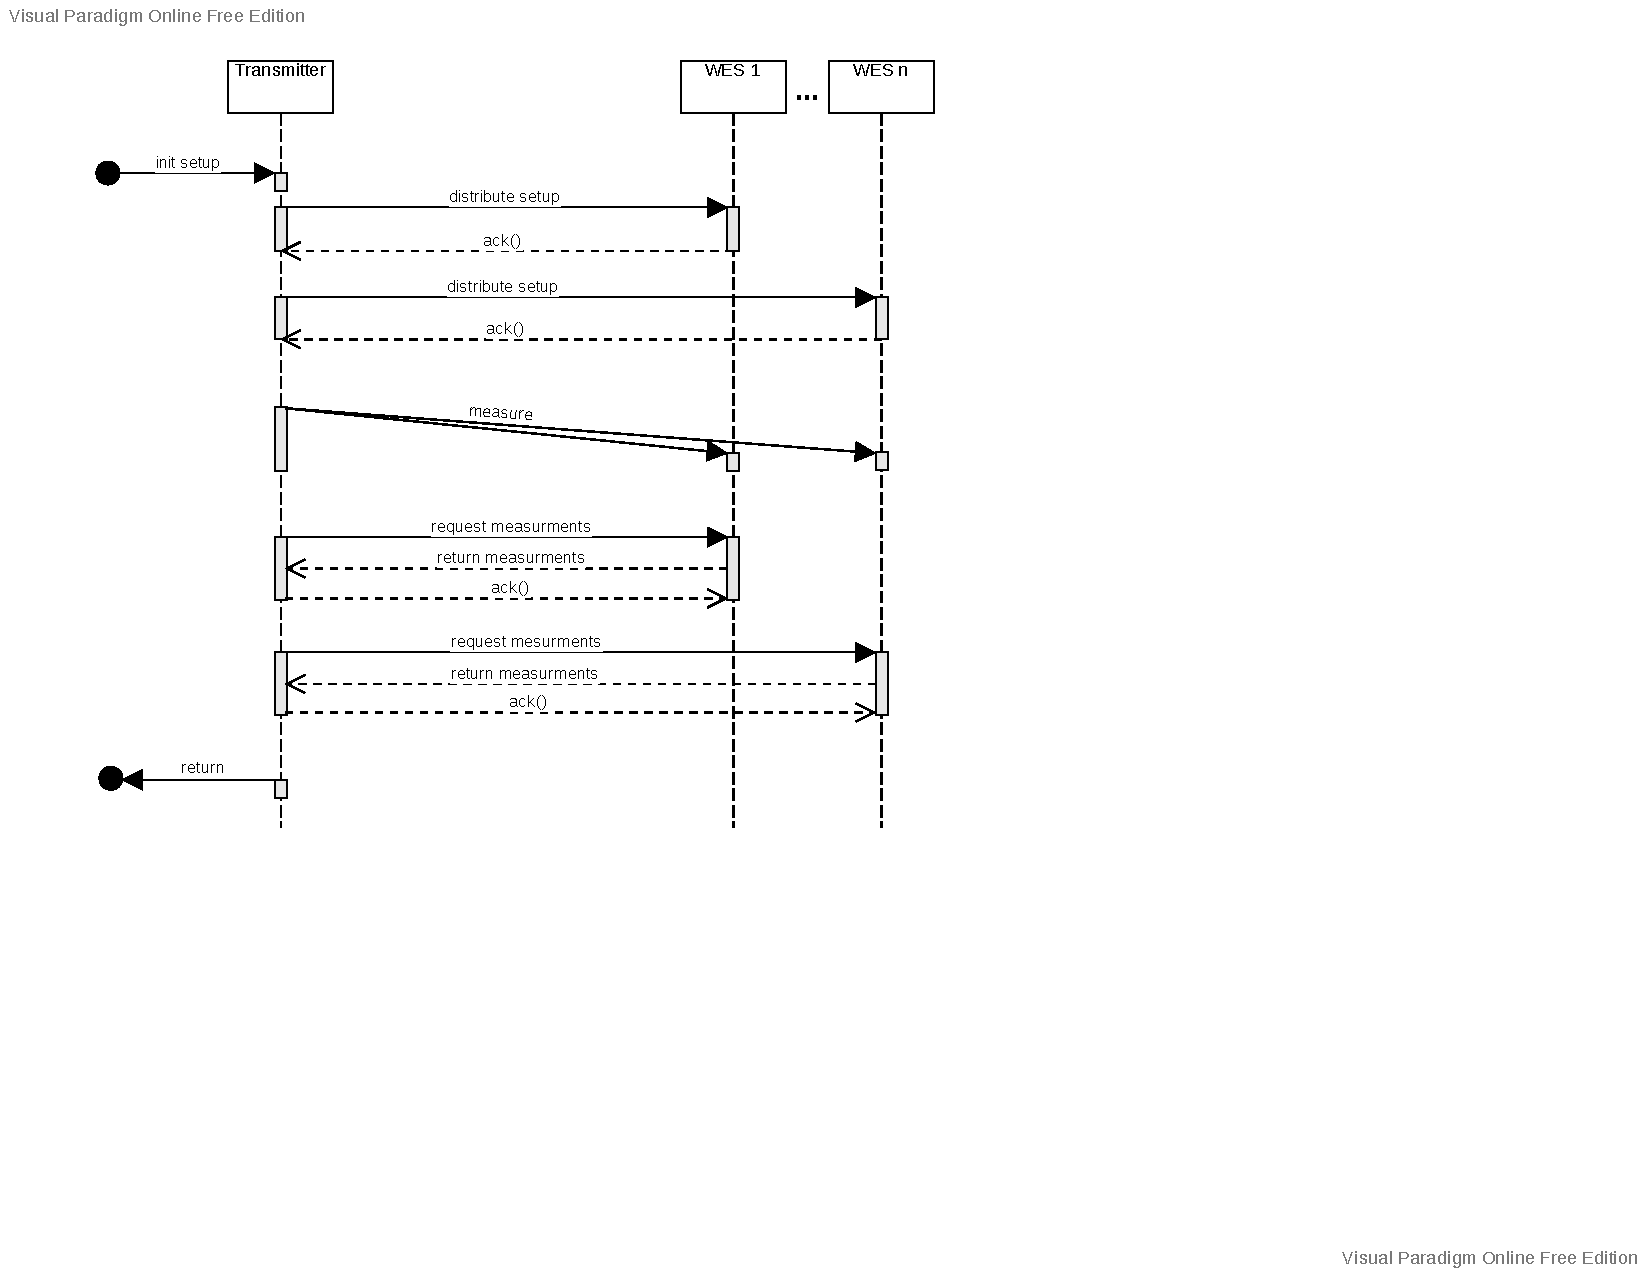
\includegraphics[scale=0.8]{figures/sequence_diagram.pdf}
	\caption{Sequence diagram of the measurment}
	\label{fig:sequenceDiagram}
\end{figure}

\begin{sequencediagram}
	\newinst{c}{:computer}
	\newthread{t}{:Transmitter}
	\newinst[2]{w}{:WES 1}
	\newinst{n}{:WES n}

	% give test vector to transmitter via serial
	% \begin{call}{c}{testVector()}{t}{ack()}
	\mess{c}{Test Parameter}{t}

	% \begin{sdblock}{}{distribute test parameter}
	\begin{call}{t}{Test Parameter}{w}{ack()}
	\end{call}
	\begin{call}{t}{Test Parameter}{n}{ack()}
	\end{call}
	% \end{sdblock}

	\mess[1]{t}{measurments}{w}
	\mess[1]{t}{measurments}{n}	

	\begin{call}{t}{request measurment}{w}{ack()}
	\end{call}
	\begin{call}{t}{request measurment}{n}{ack()}
	\end{call}
	% \begin{call}{t}{function()}{wn}{ack()}
	% \end{call}
	\mess{t}{Test Results}{c}

\end{sequencediagram}